%%%%%%%%%%%%%%%%%%%%%%%%%%%%%%%%%%
\section{Introduction}
%%%%%%%%%%%%%%%%%%%%%%%%%%%%%%%%%%

%A significant fraction of proton--proton ($pp$) collisions at the LHC involves quasi-real photon interactions.

Recently, a precise photon distribution inside the proton has been evaluated in Ref.~\cite{Manohar:2016nzj}.
This LUXqed approach provides a model-independent determination of the photon parton distribution function (PDF) inside the proton
and  it is based on proton structure function and elastic form factor fits in electron--proton scattering.

Thanks to the large fluxes of photons from the Pb ion, the $p+\textrm{Pb}$ collision configuration

The exclusive $\gamma\gamma\rightarrow\ell\ell$ process has been measured in $pp$ collisions by ATLAS~\cite{Aad:2015bwa,Aaboud:2017oiq}, CMS~\cite{Chatrchyan:2011ci,Chatrchyan:2012tv} and recently by CMS+TOTEM~\cite{Cms:2018het} collaborations.


\begin{figure}[h!]
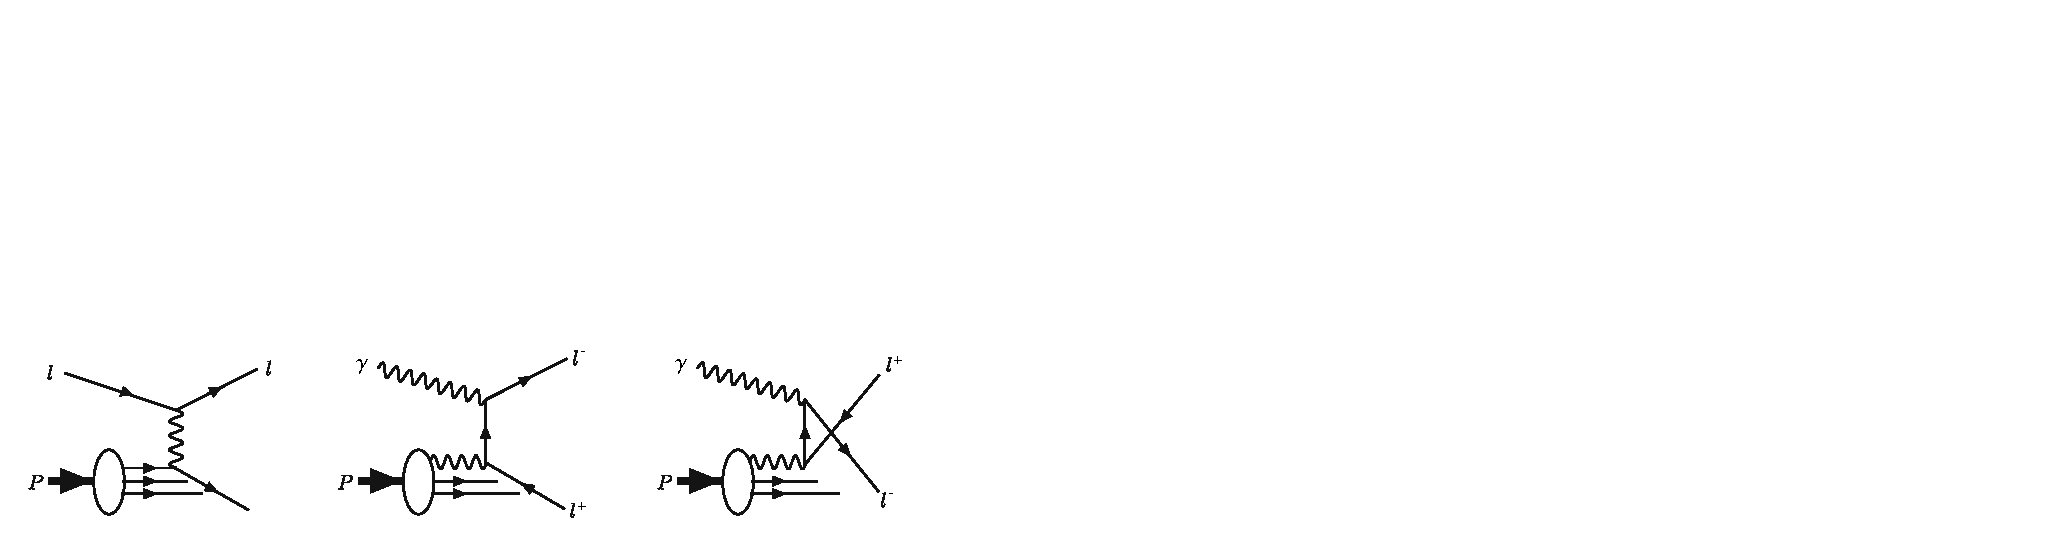
\includegraphics[width=1.\textwidth]{figures/dis_to_photon.pdf}
 \put(-400,-3){{\footnotesize(a)}}
 \put(-246,-3){{\footnotesize(b)}}
\put(-90,-3){{\footnotesize(c)}}
\caption{Schematic graphs for deep inelastic scattering, $\ell p\rightarrow \ell X$ (a) and photon-induced dilepton prodcution, $\gamma p\rightarrow \ell\ell X$, in $t$-channel (b) and $u$-channel (c).}
\label{fig:diagrams}
\end{figure}


As the signal process does not involve the exchange of color with the photon-emitting nucleus, no significant particle production is expected in the rapidity region between the dilepton system and the nucleus. 
The photon-emitting nucleus is also expected to produce no neutrons because the photons couple to the entire nucleus. 
Thus a combination of a rapidity gap and zero neutrons in the same direction provide straightforward criteria to identify these events experimentally. 


